\section{Question 1}

\subsection{The Question}

\begin{flushleft}

Using the data from A9:

- Consider each row in the blog-term matrix as a 500 dimension vector, 
corresponding to a blog.  

- From chapter 8, replace numpredict.euclidean() with cosine as the 
distance metric.  In other words, you'll be computing the cosine between
vectors of 500 dimensions.  

- Use knnestimate() to compute the nearest neighbors for both:

http://f-measure.blogspot.com/
http://ws-dl.blogspot.com/

for k={1,2,5,10,20}.

\end{flushleft}


\subsection{The Answer}
A function for the cosine similarity was made based off the definition of the dot product. This was used with the nnestimate() function

\lstset{
    language=Bash,
    label=code:q1,
    caption={Python script that computes kNN based on cosine similarity}
}
\lstinputlisting{../q1/q1.py}



\begin{figure}
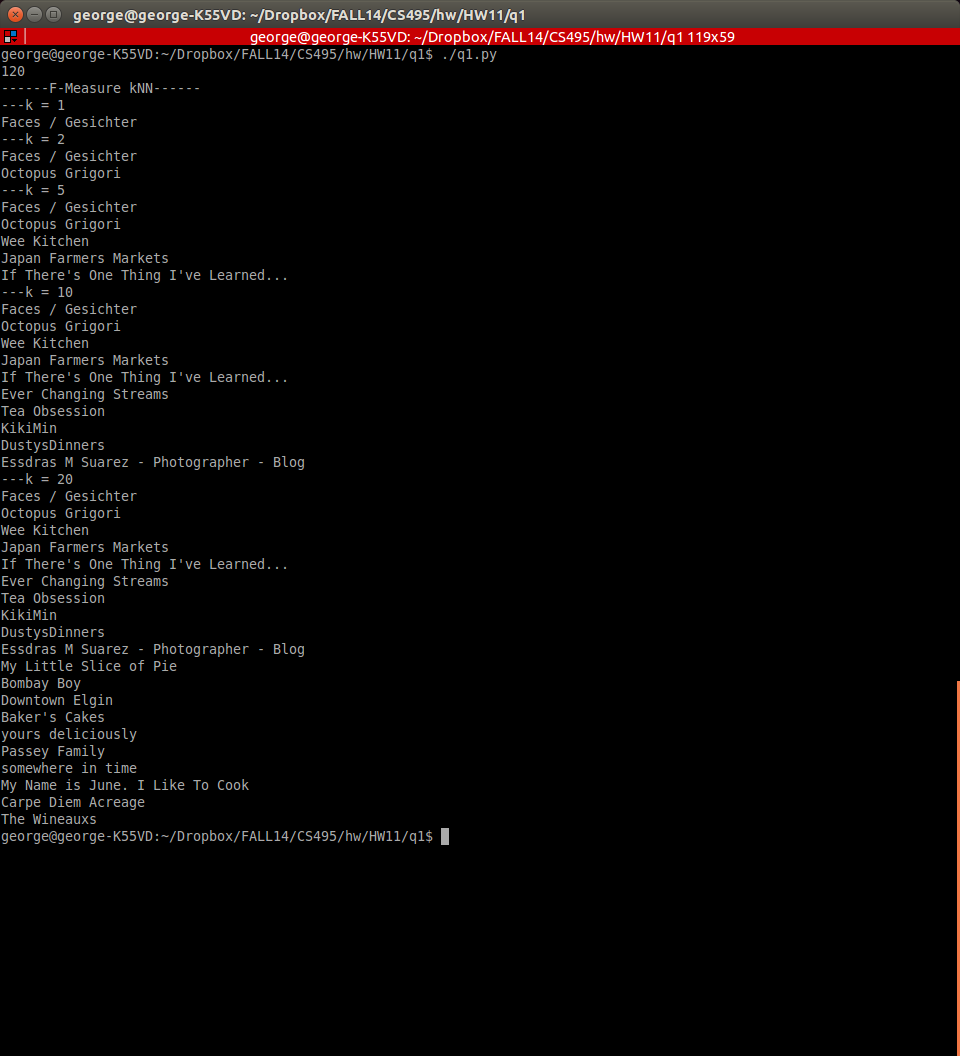
\includegraphics[width=\textwidth]{fm}
\caption{Clustings for the F-Measure blog}
\end{figure}


\begin{figure}
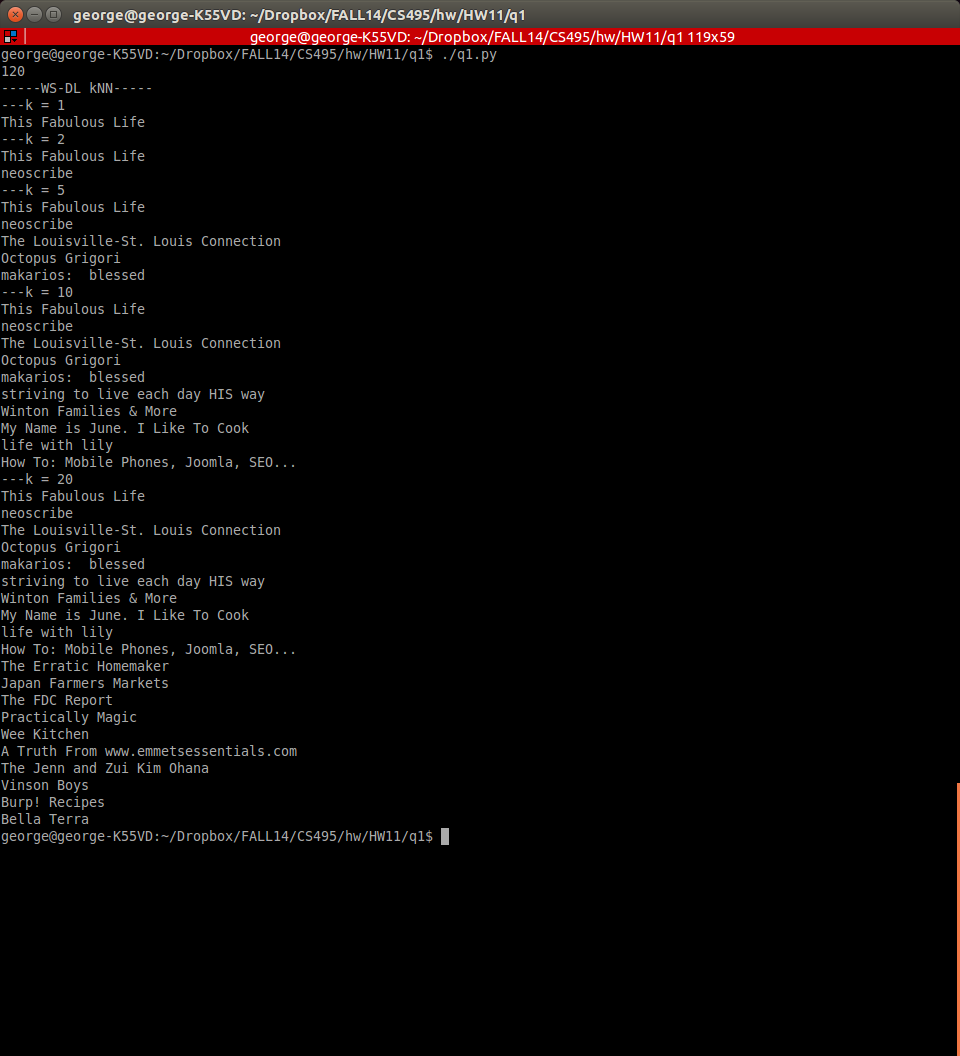
\includegraphics[width=\textwidth]{ws}
\caption{CLusterings for the WS-DL blogs}
\end{figure}




